
\chapter{Free Energy and Related Thermodynamic Quantities\label{chpt:thermodynamic-quantities}}

The solvation free energy is the most important property that we seek;
as shown in previous sections, it can be calculated by the minimization
of free energy functional $\mathcal{F}[\rho]$. Here is a discussion
about some corrections needed for charged solutes and some related
thermodynamic quantities that can be obtained directly from the solvation
free energy.

The solvation properties often involve the three-dimensional microscopic
structure of the solvent around the dissolved molecule, as well as
thermodynamic quantities such as the enthalpy, entropy, and free
energy of solvation {[}ref gubbins{]} pKa {[}ref{]}.

The solvation properties can be determined if the two principle properties, free energy and structure,
are accurately calculated. In this thesis,
we focus on these two aspects.


\section{Free energy correction for a single ion}

In the calculation of external potential as well as the total solvation
free energy, the use of different conventions can lead to a charge-independent
offset, which introduces error for charged solutes \citep{Kastenholz_2006_I,Kastenholz_2006_II,Hunenberger_book}.
This offset is mainly caused by two sources: (1) resulting from the use of
a finite system size; in our case, a system with cubic periodic
boundary conditions, which presents artificial interactions between
the ion and its own periodic copies, as well as between the solvent
and the periodic copies of the ion (Type-B in \citep{Kastenholz_2006_II});
(2) owing to the choice of convention for summing up the contributions
of solvent charges to the electrostatic potential in the sample system
(Type-C in \citep{Kastenholz_2006_II}).


\subsection{Correction of type B}

Type B correction should be added for systems with finite size or
periodic boundary conditions, accounting for the error in the solvent
polarization \marginpar{Another way to evaluate this error is to make a numerical extrapolation
of the inverse of the box size $\left(1/L\right)$; it is more accurate
but demands much more calculation.}
\begin{equation}
\Delta G_{B}=\frac{1}{8\pi\varepsilon_{0}}\left(1-\varepsilon^{-1}\right)\frac{q^{2}}{L}\left[\xi+\frac{4\pi}{3}\left(\frac{R_{\mathrm{I}}}{L}\right)^{2}-\frac{16\pi}{45}\left(\frac{R_{\mathrm{I}}}{L}\right)^{5}\right]\label{eq:corr-B}
\end{equation}
where

\begin{tabular}{cl}
 $\varepsilon_{0}$ & is the vacuum permittivity;\tabularnewline
$\varepsilon$ is the solvent permittivity (dielectric constant);\tabularnewline
$q$ & is the solute charge;\tabularnewline
$L$ & \textcolor{red}{is the box length};\tabularnewline
$R_{\mathrm{I}}$ & is the ionic radius;\tabularnewline
$\xi$ & \textcolor{red}{is the energy per particle in a simple cubic lattice,}
$\xi\simeq-2.837297$ \citep{nijboer}.\tabularnewline
 & \tabularnewline
\end{tabular} 

As $R_{\mathrm{I}}$ is significantly smaller than the size of the
computational box, i. e. $R_{\mathrm{I}}\ll L$, its quadratic as
well as higher order of $\left(R_{\mathrm{I}}/L\right)$ is considered
negligible, thus eq. (\ref{eq:corr-B}) becomes
\begin{equation}
\Delta G_{\mathrm{B}}=\frac{\xi}{8\pi\varepsilon_{0}}\left(1-\varepsilon^{-1}\right)\frac{q^{2}}{L}
\end{equation}
\textcolor{red}{It links to Born correction}.


\subsection{Correction of type C}

Type-C corrections are needed when the systems to be compared use different
electrostatic summation schemes: on the basis of point charges within
entire solvent molecules (M scheme) or on the basis of individual
point charges (P scheme), shown in figure \ref{fig:IQ-model-som-scheme}
(c) and (d), which brings a fixed free energy difference at the boundary.

\begin{figure}[h]
\begin{centering}
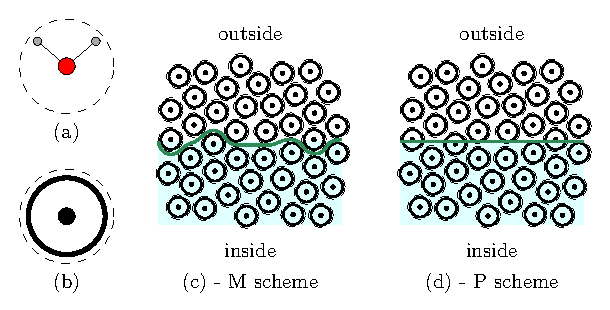
\includegraphics{_figure/ion_correction}
\par\end{centering}

\caption [IQ model and summation scheme]{IQ model and summation scheme. (a) The solvent molecule. (b) The
equivalent isotropic quadrupole (IQ) fluid model. (c) In the M scheme,
one evaluates the Coulombic potential generated by the solvent charges
belonging to all molecules within the boundary. (d) In the P scheme,
one evaluates the Coulombic potential generated by all solvent charges
within the boundary.\label{fig:IQ-model-som-scheme}}
\end{figure}


It can be deduced analytically by considering the solvent as a \textcolor{red}{canonical
ensemble} under the orientational disorder limit (ODL) \citep{Kastenholz_2006_I},
which becomes an isotropic quadrupole (IQ) fluid, whose solvent molecule
(figure \ref{fig:IQ-model-som-scheme} (b)) possesses the same quadrupole
trace $\gamma$ \marginpar{$\gamma$ which is elsewhere referred to as the spheropole moment \citep{Saunders_1992,Maschio_2012},
that is, the spherical component of the quadrupole moment, and is
invariant with respect to rotations.}
\begin{equation}
\gamma=\mathrm{tr}(\mathbf{\mathcal{Q}})=\mathcal{Q}_{xx}+\mathcal{Q}_{yy}+\mathcal{Q}_{zz}
\end{equation}
where the quadrupole moment of the solvent molecule can be calculated
by its definition \citep{Multipole}:
\begin{equation}
\mathcal{Q}_{ij}=\int_{V}r_{i}r_{j}\rho(\mathbf{r})\mathrm{d}v=\sum_{\alpha=1}^{N}q^{(\alpha)}r_{i}^{(\alpha)}r_{j}^{(\alpha)}
\end{equation}


It can be shown that the charge density of a solvent located within the
boundary of a sample system vanishes everywhere except at the boundary
in the M scheme, which results in a uniform normal surface polarization.
The correction needed for\textcolor{red}{{} M scheme }is
\begin{equation}
\Delta G_{\mathrm{C}}=-q\left(1-\frac{4\pi R_{\mathrm{I}}^{3}}{3L^{3}}\right)\Delta\Phi_{\mathrm{ODL}}\label{eq:corr-C}
\end{equation}
where $\Delta\Phi_{\mathrm{ODL}}=\left(6\varepsilon_{0}\right)^{-1}\eta\gamma$,
$\eta$ being the solvent number density.

In the same way, when we consider $R_{\mathrm{I}}\ll L$, eq. (\ref{eq:corr-C})
becomes
\begin{equation}
\Delta G_{\mathrm{C}}=-\left(6\varepsilon_{0}\right)^{-1}\eta\gamma q
\end{equation}



\section{Some related thermodynamic quantities}

Thermodynamic quantities such as the internal energy, pressure, compressibility
and heat capacity are obtained as derivatives of the classical partition
function. {[}Evans poly{]}

Structure and Thermodynamic Properties of Bulk Liquids

Pressure is (virial pressure equation) 
\begin{equation}
p=\rho k_{\mathrm{B}}T-\dfrac{\rho^{2}}{2}\int\mathrm{d}\mathbf{r}g(r)\frac{r}{3}\frac{\mathrm{d}u(r)}{\mathrm{d}r}
\end{equation}


The Gibbs free energy G is simply {[}Evans 1979{]}.

$G=\mu\int\mathrm{d}\mathbf{r}\rho(\mathbf{r})$


\subsection{Solubility}


\subsection{Pressure}

enthalpy, entropy {[}3{]} pH
